\documentclass[dvipsnames,tikz]{standalone}
\usepackage{tikz}
\usepackage{cmbright}      % sansfont
\usetikzlibrary{shapes,positioning}

\tikzset{main/.style={color=black}}

\begin{document}
	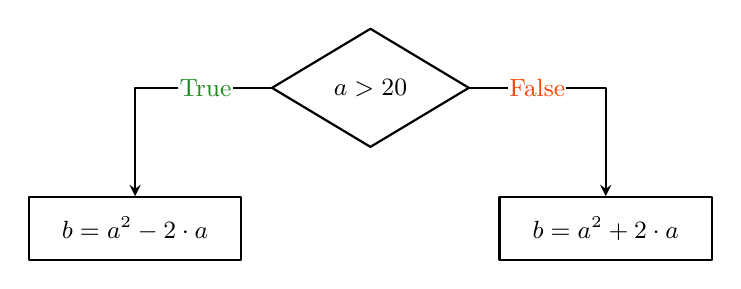
\begin{tikzpicture}[font=\small,thick, line join=bevel]
		%% Nodes
		\node[
			draw,
			main,
			diamond,
			minimum width=2.5cm,
			minimum height=1.5cm,
			outer sep = 0,
			inner sep=0] (keuze1) {$a > 20$};

		\node[xshift=-0.5cm,
			inner sep = 0,
			right=of keuze1] (false) {\color{OrangeRed}False};
		\node[xshift=0.5cm,
			inner sep = 0,
			left=of keuze1] (true) {\color{ForestGreen}True};
		
		\node[draw,
			main,
			below left=of keuze1,
			minimum width=2.7cm,
			minimum height=0.8cm] (vriest) { $b = a^2 - 2 \cdot a$ };
		\node[draw,
			main,
			below right =of keuze1,
			minimum width=2.7cm,
			minimum height=0.8cm] (dooit) { $b = a^2 + 2 \cdot a$ };
		
		%% Connections
		\draw[main] (keuze1) -- (true);
		\draw[-stealth,main] (true) -| (vriest);
		\draw[main] (keuze1) -- (false);
		\draw[-stealth, main] (false) -| (dooit);
	\end{tikzpicture}
\end{document}